Die Konstruktion wurde in 3 einzelne Teile aufgeteilt: Bodenplatte, hinterer Aufbau und Lenkung. Diese Teile sind mit wenigen Schrauben und Steckverbindungen voneinander trennbar, um den Transport und die Lagerung zu vereinfachen.\\
Der Aufbau wurde in dem 3D-Programm Inventor\textsuperscript{\cite{Inventor}} geplant und konstruiert.\\
\begin{figure}[H]
    \centering
    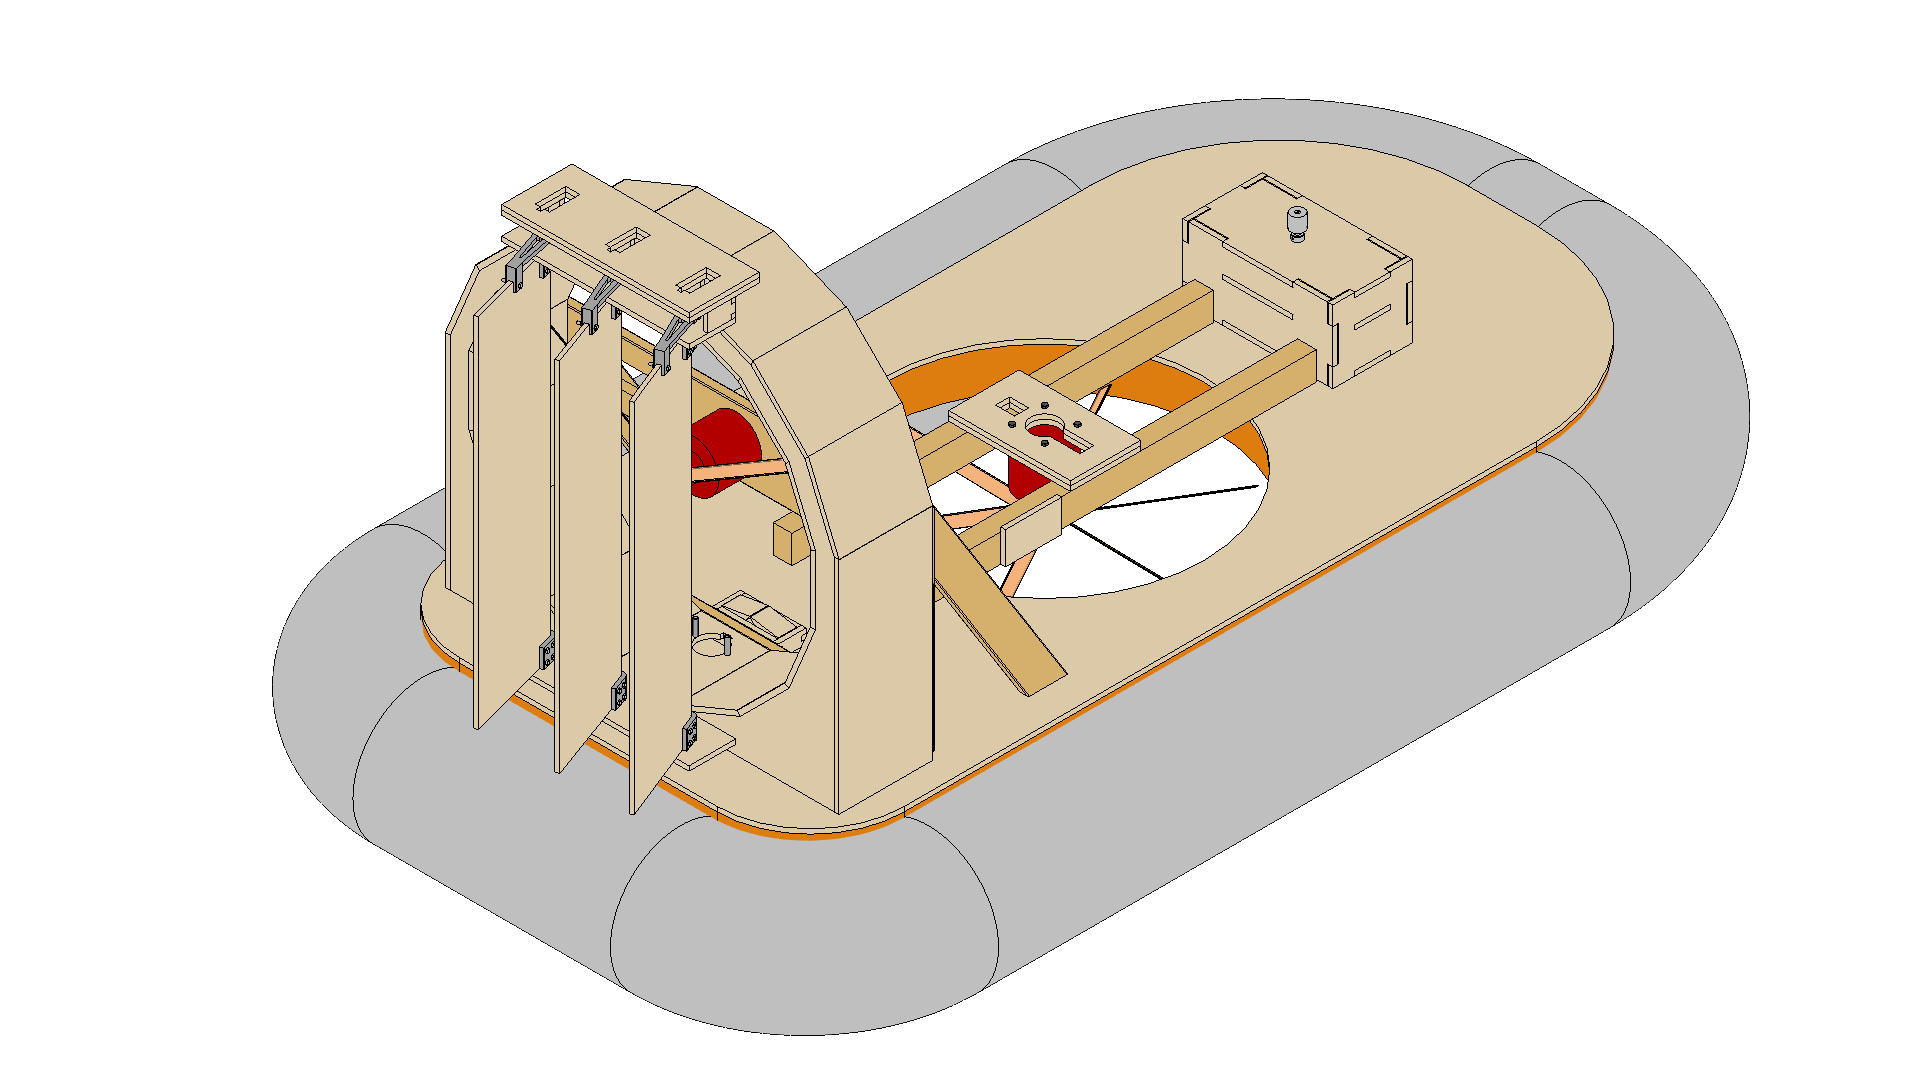
\includegraphics[width=\textwidth]{../Inventor/Luftkissenboot.png}
    \caption{Konstruktion 3D-Modell gesamt}
\end{figure}

\clearpage
\section{Bodenplatte}
Die Bodenplatte ist die Grundlage, auf welcher die anderen beiden Teile befestigt sind, und stellt die Verbindung mit dem Boot da.\\
Um die Bodenplatte möglichst leicht aber trotzdem stabil zu halten, wurde \ac{xps} in Verbindung mit Pappelsperrholz verwendet.\\
% Die Bodenplatte wurde aus 10cm dicken \ac{xps}--Platten und einer 1cm dicken Pappelsperrholzplatte zusammengesetzt. In das \ac{xps} wurden zur Verstärkung noch links und rechts 2 20x95\,mm Holzlatten eingefräst und eingeklebt.\\ 
In der Mitte der Bodenplatte wurde das Loch für den Propeller ausgeschnitten. Im \ac{xps} wurde der Lochdurchmesser so gewählt, dass der Propeller darin frei drehen kann. Der Lochdurchmesser in der Holzplatte darüber wurde um 2\,cm kleiner gewählt, um zu verhindern das am Rand des Loches die Luft direkt wieder hinausströmt.

\begin{figure}[H]
    \centering
    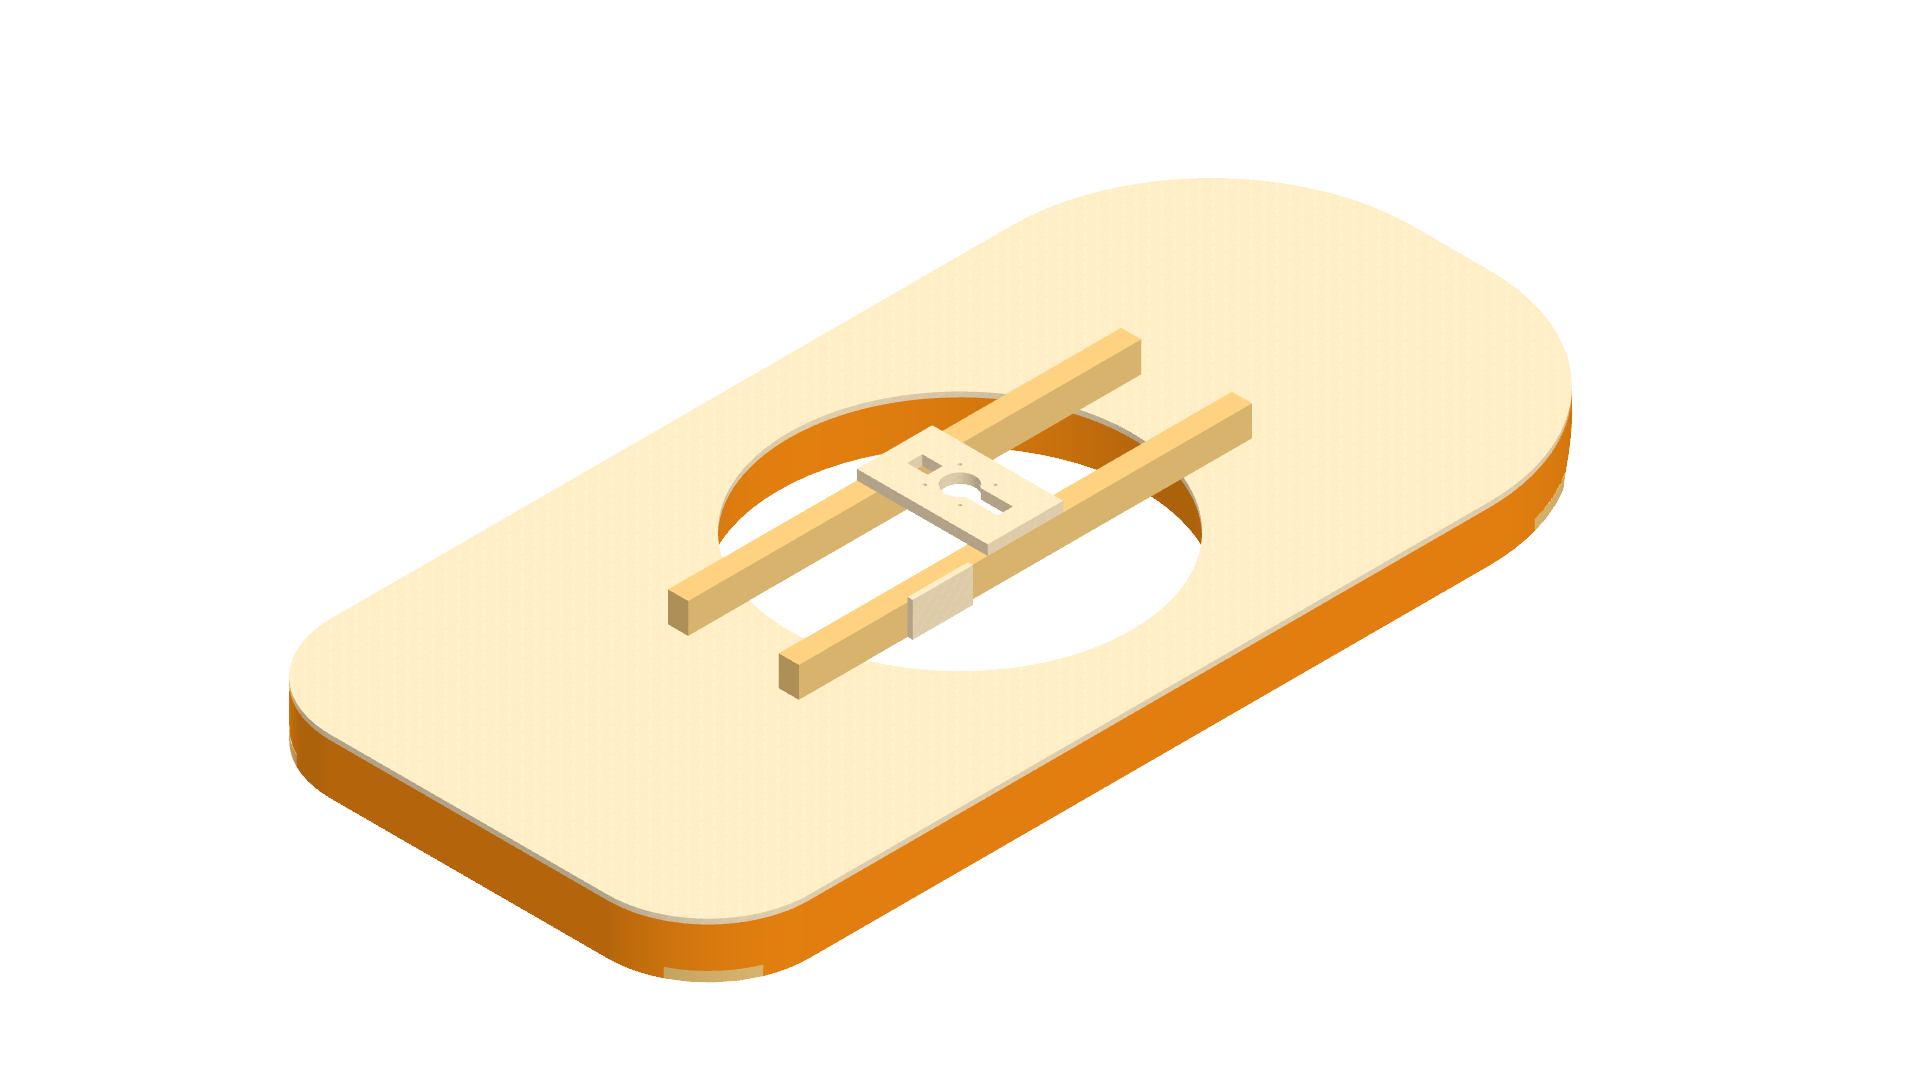
\includegraphics[width=\textwidth]{../Inventor/Bodenplatte/png/BodenplatteHauptansicht.png}
    \caption{Bodenplatte 3D-Modell\label{fig:konst:bodenplatte:gesamt}}
\end{figure}

\clearpage
\subsection{Stückliste}
\begin{table}[H]
    \centering
    \begin{tabular}{|c|M{4.5cm}|M{3.5cm}|c|c|}
        \hline
        \textbf{Stk} & \textbf{Name} & \textbf{Material} & \textbf{Herstellung} & \textbf{Abbildung}\\\hline
        1 & Bodenplatte Pappel  & 10mm Pappel & Stichsäge & \ref{fig:bodenplatte:skizze:BodenplattePappel}\\\hline
        1 & Bodenplatte XPS & 100mm \ac{xps} & Messer & \ref{fig:bodenplatte:skizze:BodenplatteXPS1}, \ref{fig:bodenplatte:skizze:BodenplatteXPS2}\\\hline
        1 & Verstärkung Holzlatte links & Holzlatte Fichte 20x90mm & Kappsäge & \ref{fig:bodenplatte:skizze:VHOLZL}\\\hline
        1 & Verstärkung Holzlatte rechts & Holzlatte Fichte 20x90mm & Stichsäge & \ref{fig:bodenplatte:skizze:VHOLZR}\\\hline
        2 & Staffel Motorhalterung & Staffel gehobelt 40x60mm & Stichsäge & \ref{fig:bodenplatte:skizze:Staffel}\\\hline
        2 & Platte Motorhalterung & 10mm Pappel & LaserCutter & \ref{fig:bodenplatte:skizze:Motorhalterung}\\\hline
        1 & Platte Motorregler-Halterung & 10mm Pappel & LaserCutter & \ref{fig:bodenplatte:skizze:Motorreglerhalterung}\\\hline
        1 & Gitter unten & Lochplatte & Gekauft & \ref{fig:konst:gitter} \\\hline
    \end{tabular}
    \caption{Stückliste Bodenplatte}
    \label{tab:konst:bodenplatte:stueckliste}
\end{table}

\clearpage
\subsection{Inventor}
\begin{figure}[H]
    \centering
    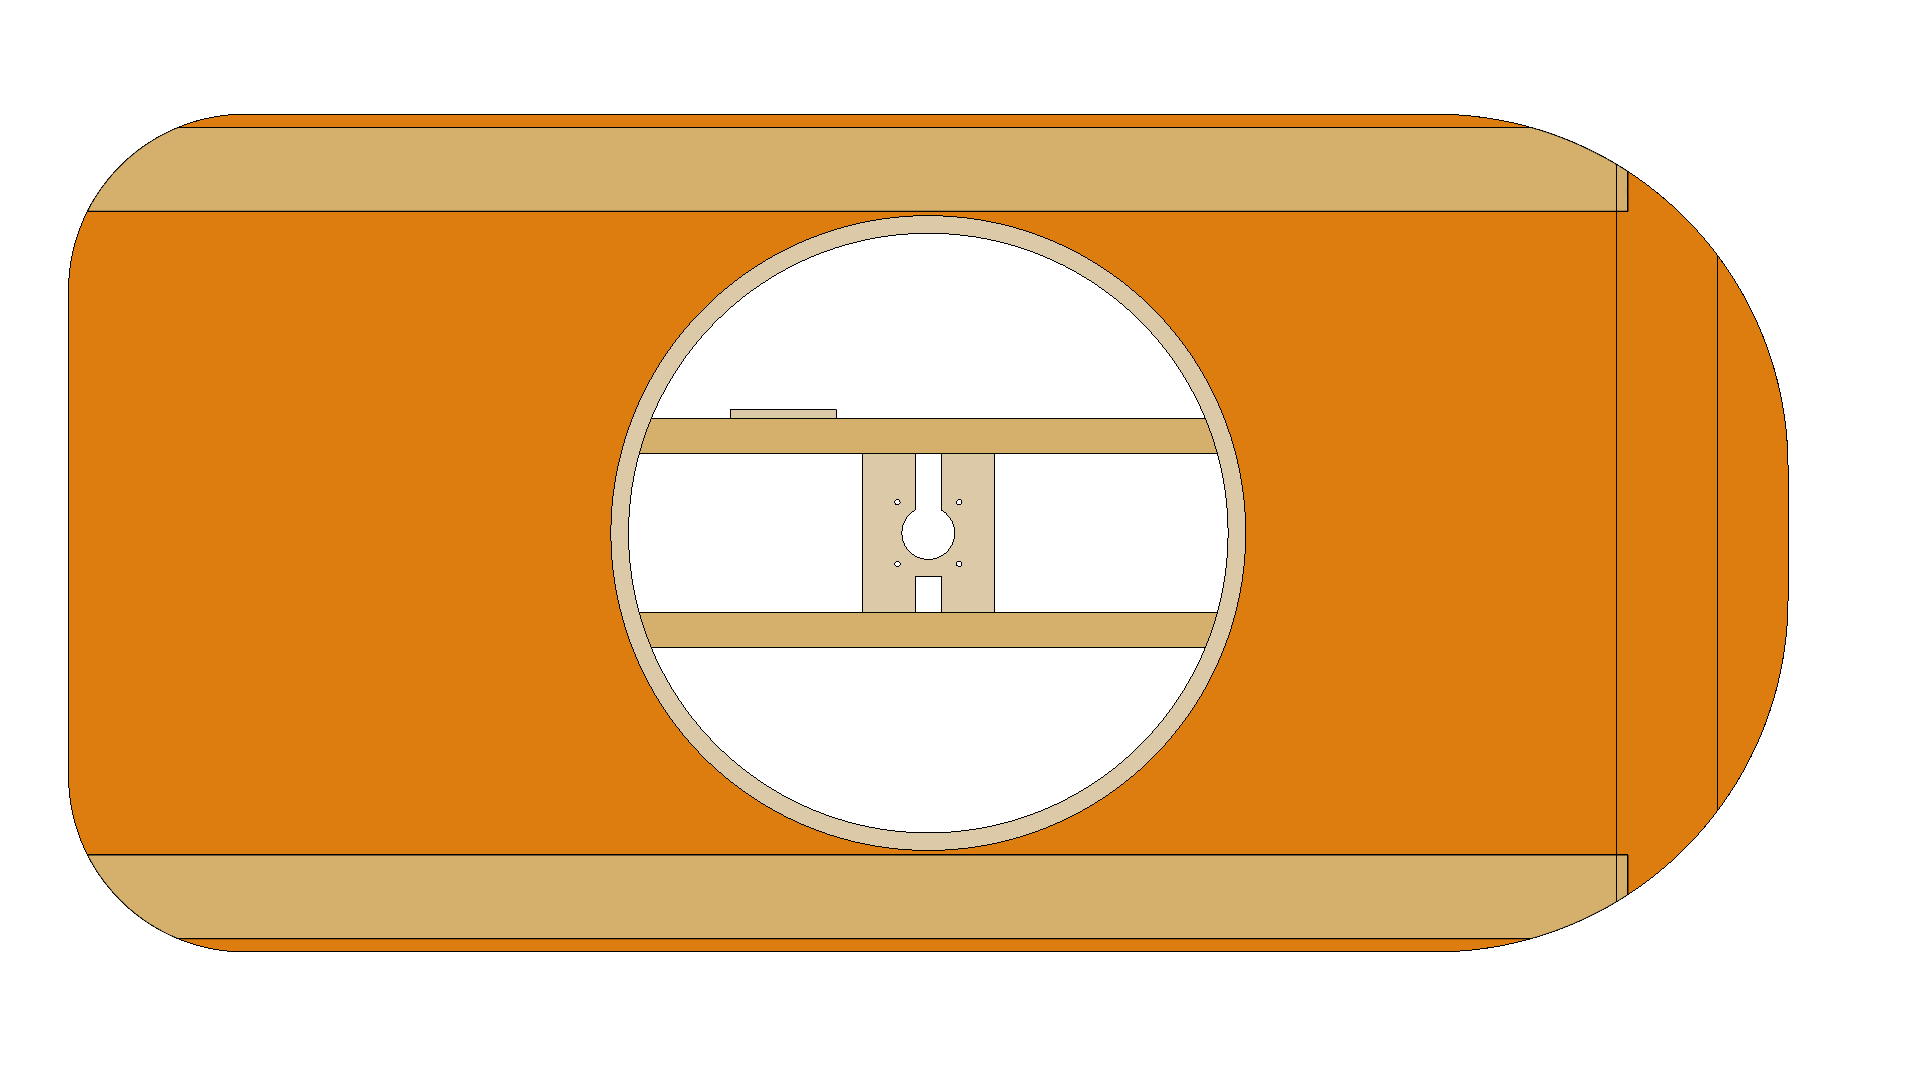
\includegraphics[width=.92\textwidth]{../Inventor/Bodenplatte/png/Bodenplatte_unten.png}
    \label{fig:konst:bodenplatte:inventor1}
    \caption{Bodenplatte Ansicht unten}
\end{figure}
\begin{figure}[H]
    \centering
    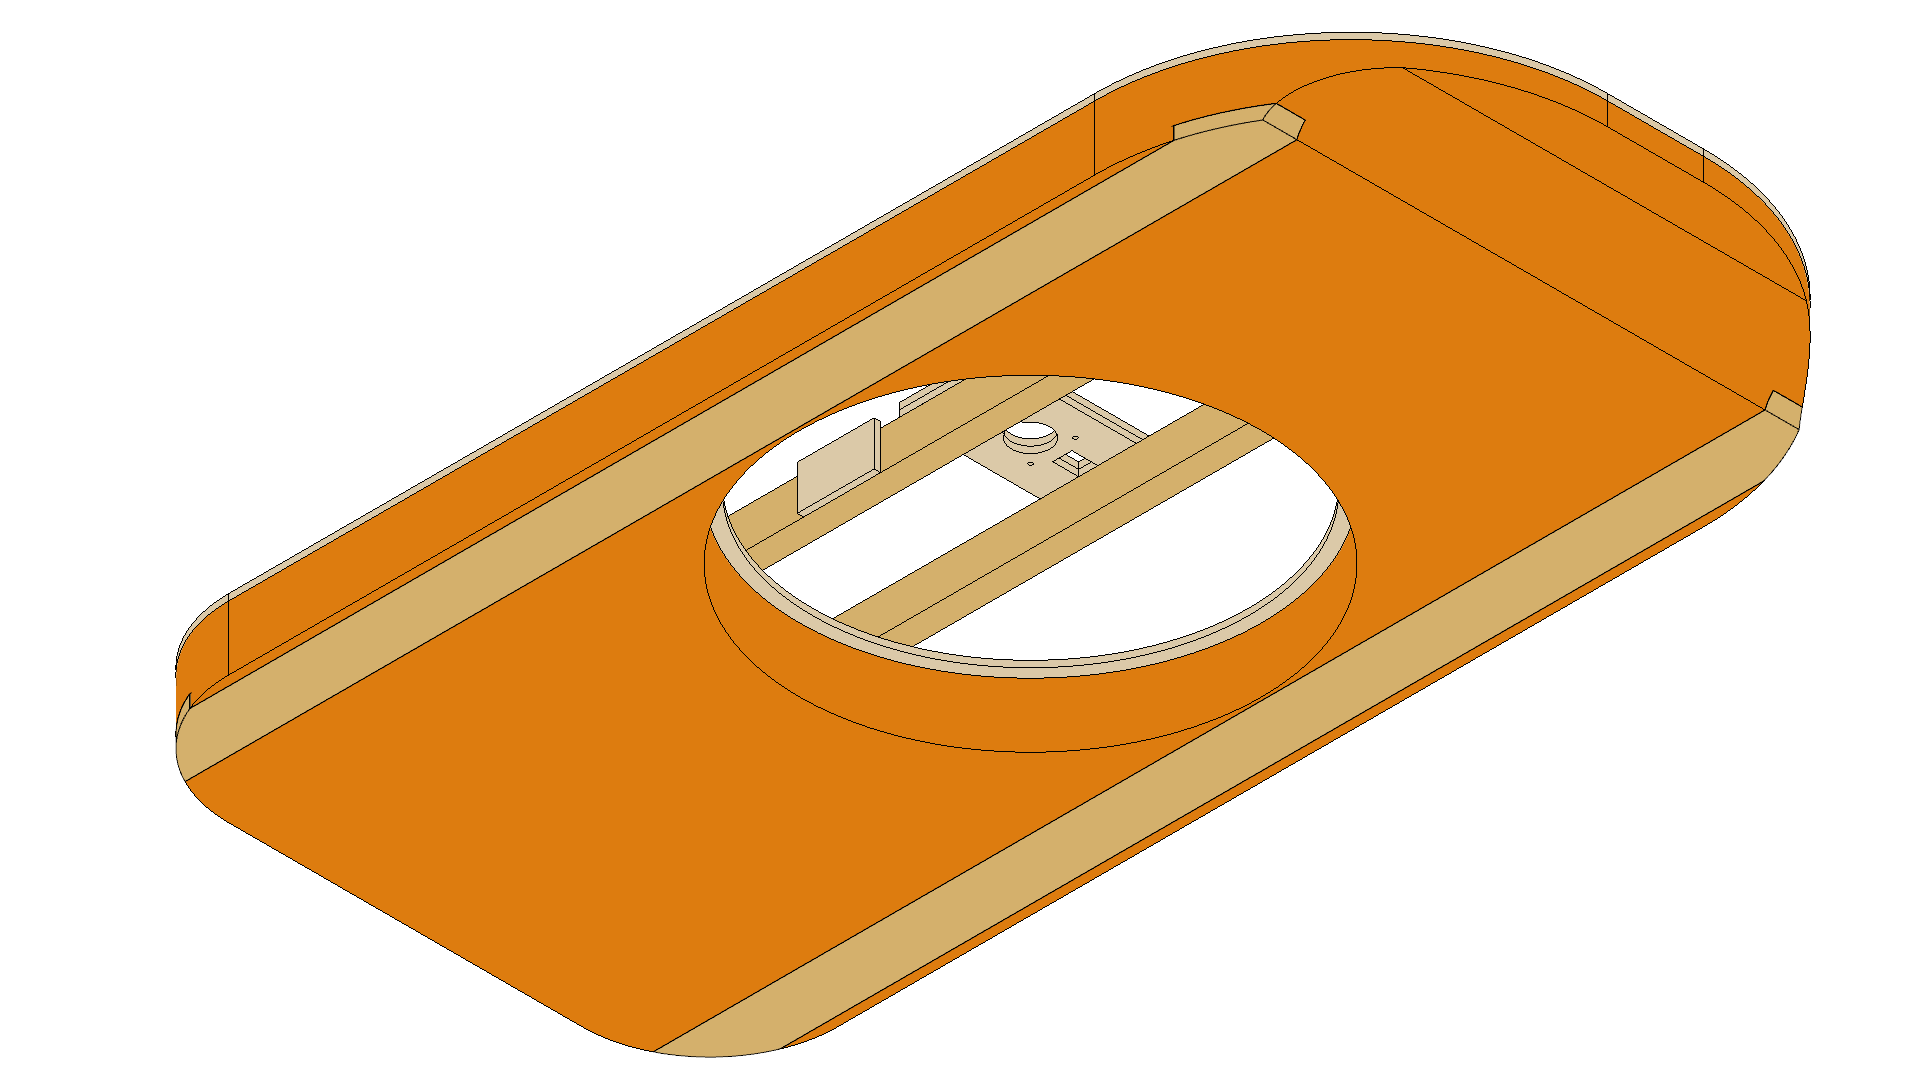
\includegraphics[width=.92\textwidth]{../Inventor/Bodenplatte/png/Bodenplatte_seitlich.png}
    \label{fig:konst:bodenplatte:inventor2}
    \caption{Bodenplatte Ansicht unten seitlich}
\end{figure}

\begin{landscape}
    \includeSkizze{../Inventor/Bodenplatte/Zeichnung/Bodenplatte-Holz.pdf}{Bodenplatte Pappel}{fig:bodenplatte:skizze:BodenplattePappel}{1}
    \clearpage

    \includeSkizze{../Inventor/Bodenplatte/Zeichnung/Bodenplatte-XPS.pdf}{Bodenplatte XPS 1}{fig:bodenplatte:skizze:BodenplatteXPS1}{1}
    \clearpage
    \includeSkizze{../Inventor/Bodenplatte/Zeichnung/Bodenplatte-XPS.pdf}{Bodenplatte XPS 2}{fig:bodenplatte:skizze:BodenplatteXPS2}{2}
    \clearpage

    \includeSkizze{../Inventor/Bodenplatte/Zeichnung/HolzLatteLinks.pdf}{Verstärkung Holzlatte links}{fig:bodenplatte:skizze:VHOLZL}{1}
    \clearpage

    \includeSkizze{../Inventor/Bodenplatte/Zeichnung/HolzLatteRechts.pdf}{Verstärkung Holzlatte rechts}{fig:bodenplatte:skizze:VHOLZR}{1}
    \clearpage

    \includeSkizze{../Inventor/Bodenplatte/Zeichnung/40x60Staffel.pdf}{Staffel Motorhalterung}{fig:bodenplatte:skizze:Staffel}{1}
    \clearpage

    \includeSkizze{../Inventor/Bodenplatte/Zeichnung/Motorhalterung.pdf}{Motorhalterung}{fig:bodenplatte:skizze:Motorhalterung}{1}
    \clearpage

    \includeSkizze{../Inventor/Bodenplatte/Zeichnung/HalterungMotorregler.pdf}{Motorregler-Halterung}{fig:bodenplatte:skizze:Motorreglerhalterung}{1}
    \clearpage

\end{landscape}
\cleardoublepage

\subsection{Gitter}
Das untere Gitter musste so stabil gewählt werden, dass der Fahrer problemlos darauf sitzen kann. Gleichzeitig muss es aber auch genug Luft durchlassen.\\
Wir haben uns deshalb für ein Lochblech mit quadratischen Löchern mit 5mm Seitenlänge entschieden. Der Steg zwischen den Löchern ist 3mm breit, insgesamt ist das Gitter 73x73cm groß.\\
\begin{figure}[H]
    \centering
    \missingfigure{Foto Gitter machen von oben}
    \caption{Foto Gitter \label{fig:konst:gitter}}    
\end{figure}

\clearpage
\subsection{Zusammenbau}
Die \ac{xps}-Platte wurde aus 4 einzelnen 100mm dicken \ac{xps}-Platten zusammengeklebt und mit einem Messer zugeschnitten. Die Schlitze für die Holzlatten wurden mit einer Oberflächenfräse eingefräst und die Holzlatten (\autoref{fig:bodenplatte:skizze:VHOLZL} \&\ \autoref{fig:bodenplatte:skizze:VHOLZR}) wurden mit Silikon eingeklebt.\\
Die Pappelsperrholzplatte wurde mit 8 M8x120mm Schrauben mit der \ac{xps}-Platte verschraubt.\\
Danach wurde das Metallgitter montiert und die Staffeln zur Motorhalterung wurden darüber geleimt und geschraubt.\\
Um die anderen beiden Teile befestigen zu können, wurden einige Winkel an der Bodenplatte angeschraubt -- siehe \autoref{fig:konst:Winkelverbinder}.\\
Außerdem wurde in die \ac{xps}-Platte ein Kabelkanal für eine CAN-Bus--Leitung, eine Leitung für den Not-Aus sowie eine für den Precharge-Button eingefräst. Dieser Kabelkanal läuft von der Lenkung bis zum hinteren Aufbau.
\begin{figure}[H]
    \centering
    \missingfigure{Foto Winkelverbinder machen (neu für DSC\_8596)}
    \caption{Bodenplatte Winkelverbinder\label{fig:konst:Winkelverbinder}}    
\end{figure}
\begin{figure}[H]
    \centering
    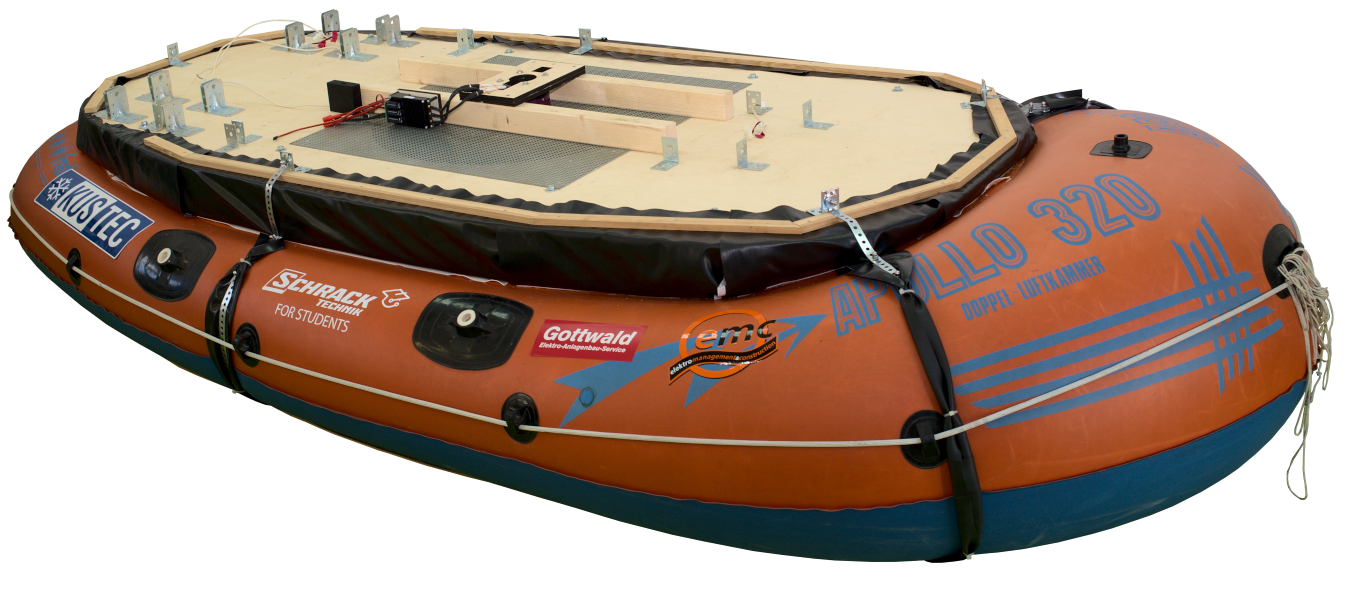
\includegraphics[width=.99\textwidth]{Fotos/Konstruktion/DSC_8622.png}
    \caption{Zusammenbau Bodenplatte \label{fig:konst:bodenplatte_zusammenbau}}    
\end{figure}
\begin{figure}[H]
    \centering
    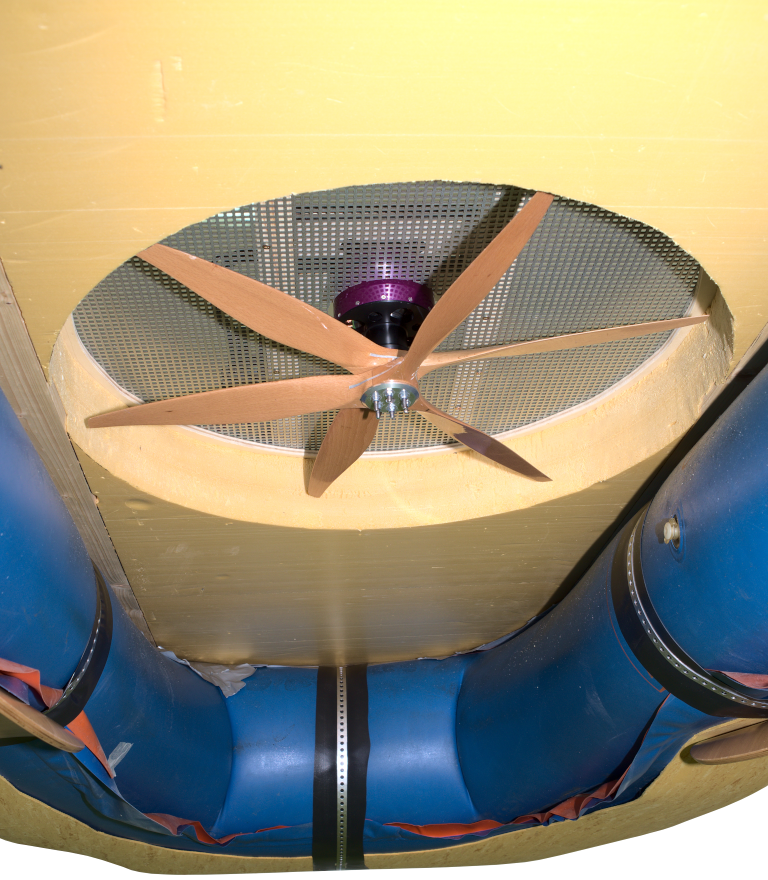
\includegraphics[width=.99\textwidth]{Fotos/Konstruktion/DSC_8600.png}
    \caption{Zusammenbau Bodenplatte Sicht von unten}    
\end{figure}

\subsection{Montage am Boot}
Die Bodenplatte soll möglichst luftdicht mit dem Schlauchboot verbunden werden. Um dies zu erreichen, wurde eine Teichfolie mit doppelseitigem Klebeband am Boot angeklebt und an der Holzplatte mit einer Leiste angeschraubt.\\
Um die Unterseite des Bootes beim Bremsen zu schützen, wurde ein Stück aus einer Bodenplatte ausgeschnitten und mit Pattex Kraftkleber an das Boot geklebt.\\
Um ein Verrutschen der Konstruktion zu verhindern, wurde die Bodenplatte zusätzlich mit einem Lochband am Boot befestigt -- siehe \autoref{fig:konst:fotoLochband}
\begin{figure}[H]
    \centering
    \includegraphics[width=.99\textwidth]{Fotos/Konstruktion/DSC_8616.png}
    \caption{Befestigung Lochband\label{fig:konst:fotoLochband}}    
\end{figure}
 

\clearpage
\section{Aufbau hinten}
Der hintere Aufbau beinhaltet den Motor für den Vortrieb sowie die Fahnen zum Lenken. Die 3 Fahnen werden von 3 einzelnen Servos angesteuert.\\ Außerdem sind die Akkus und die Kupferschienen zur Stromverteilung im unteren Teil des Aufbaus versteckt. Um die Akkus zugänglich zu machen, sind die zwei äußeren Platten (\autoref{fig:Aufbau:skizze:aussengross}) aufklappbar.

\begin{figure}[H]
    \centering
    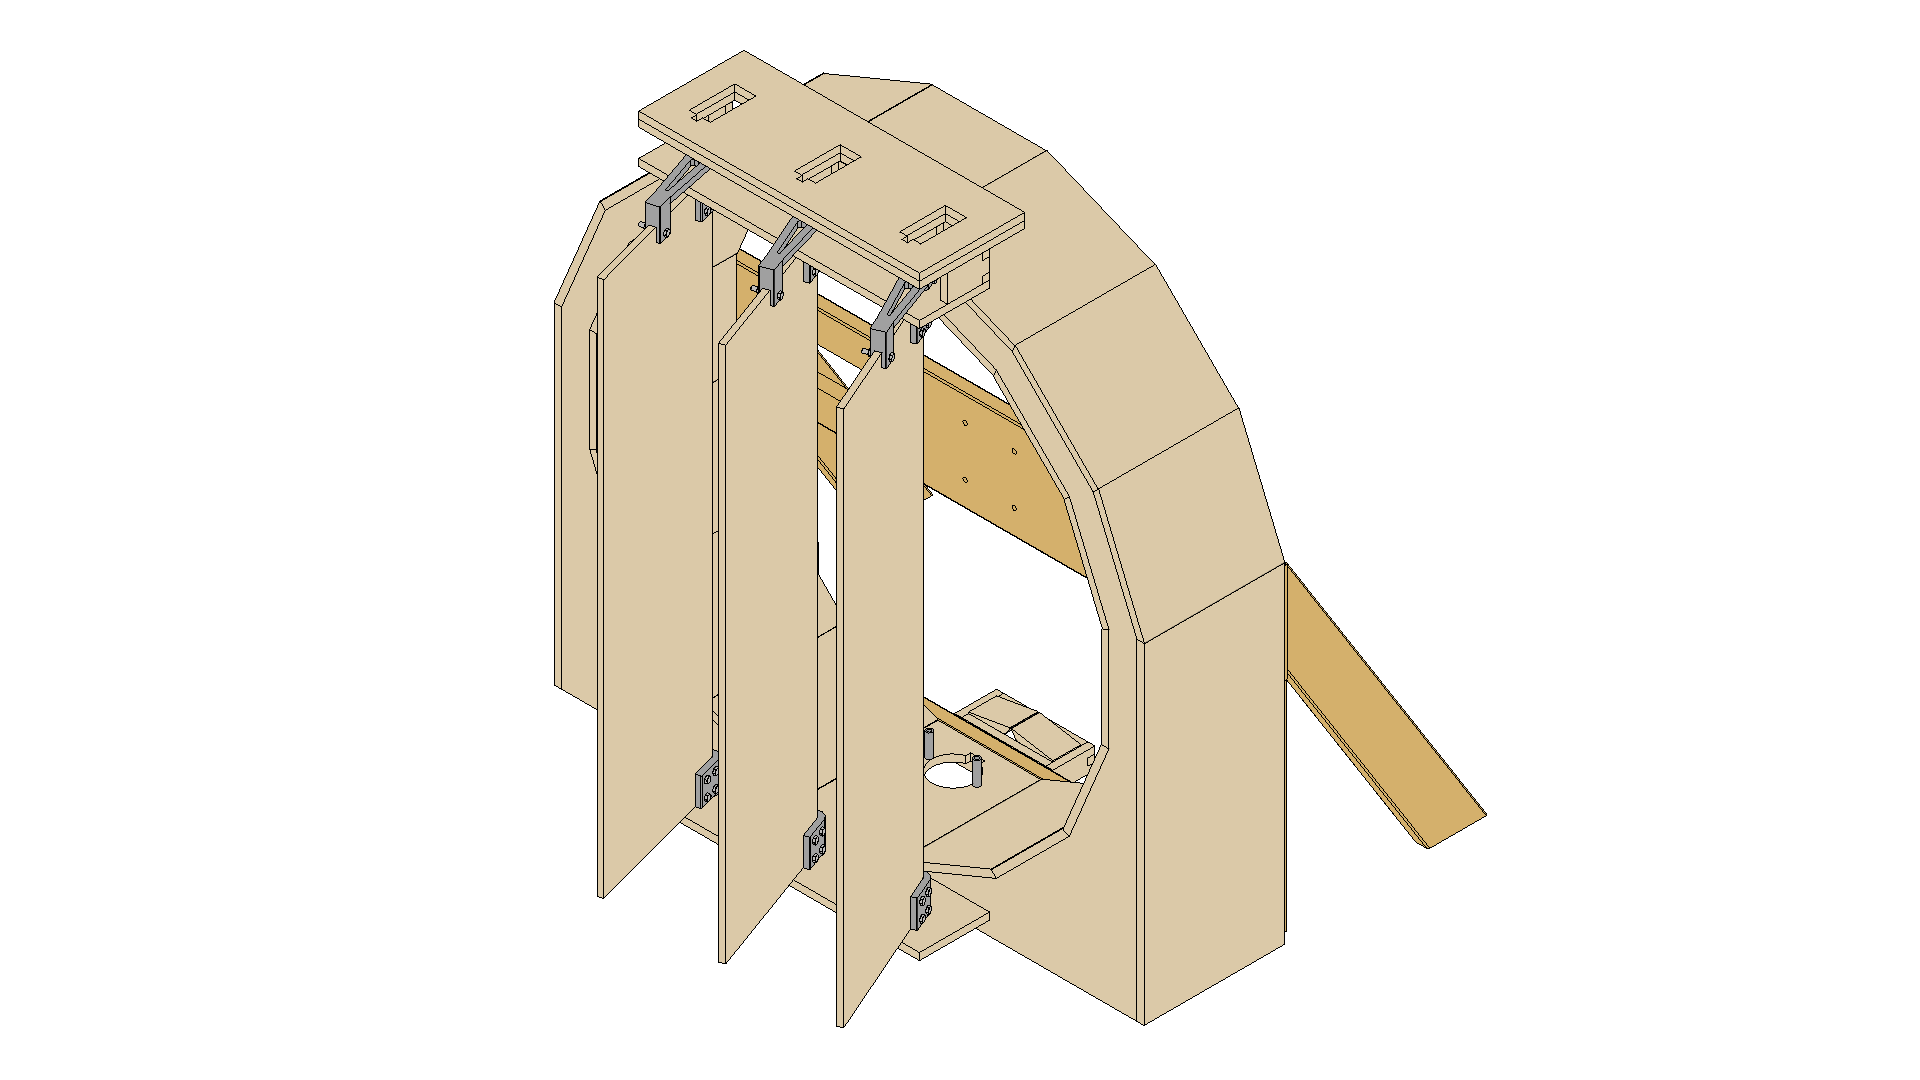
\includegraphics[width=1.1\textwidth]{../Inventor/hintererAufbau/png/hintererAufbau_hauptansicht.png}
    \label{fig:aufbau:haupt}
    \caption{hinterer Aufbau 3D-Modell}
\end{figure}

\subsection{Stückliste}
\begin{table}[H]
    \centering
    \begin{tabular}{|c|M{4.5cm}|M{3.5cm}|c|c|}
        \hline
        \textbf{Stk} & \textbf{Name} & \textbf{Material} & \textbf{Herstellung} & \textbf{Abbildung}\\\hline
        2 & Hauptplatte & 10mm Pappel & Stichsäge & \ref{fig:Aufbau:skizze:hauptplatte}\\\hline
        1 & Platte innen unten & 10mm Pappel & Stichsäge & \ref{fig:Aufbau:skizze:innenUnten}\\\hline
        14 & Platten innen 1 schräge Kante & 10mm Pappel & Handkreissäge & \ref{fig:Aufbau:skizze:innen1seite}\\\hline
        1 & Platte innen 2 schräge Kanten & 10mm Pappel & Handkreissäge & \ref{fig:Aufbau:skizze:innen2seite}\\\hline
        1 & Platte außen oben & 10mm Pappel & Stichsäge & \ref{fig:Aufbau:skizze:assenOebn}\\\hline
        4 & Platte außen 1 schräge Kante & 10mm Pappel & Handkreissäge & \ref{fig:Aufbau:skizze:aussen1seite}\\\hline
        2 & Platte außen 2 schräge Kanten & 10mm Pappel & Handkreissäge & \ref{fig:Aufbau:skizze:assen2seite}\\\hline
        2 & Platte außen Seite & 10mm Pappel & Handkreissäge & \ref{fig:Aufbau:skizze:aussengross}\\\hline
        1 & Verstärkung hinten Mitte & 10mm Pappel & Stichsäge & \ref{fig:Aufbau:skizze:vhintenmitte}\\\hline
        2 & Verstärkung hinten Unten & 10mm Pappel & Stichsäge & \ref{fig:Aufbau:skizze:vhintenunten}\\\hline
        2 & Verstärkung hinten schräg & 10mm Pappel & Stichsäge & \ref{fig:Aufbau:skizze:vhintenschraeg}\\\hline
        1 & Verstärkung unten & 10mm Pappel & Handkreissäge & \ref{fig:Aufbau:skizze:vunten}\\\hline
        2 & Servo Halter seitlich & 10mm Pappel & LaserCutter & \ref{fig:Aufbau:skizze:shs}\\\hline
        2 & Servo Halter seitlich 2& 10mm Pappel & LaserCutter & \ref{fig:Aufbau:skizze:shs2}\\\hline
        1 & Servo Halter hinten& 10mm Pappel & LaserCutter & \ref{fig:Aufbau:skizze:shh}\\\hline
        1 & Servo Halter lang& 10mm Pappel & LaserCutter & \ref{fig:Aufbau:skizze:shl}\\\hline
        2 & Servo Halter Hauptplatte& 10mm Pappel & LaserCutter & \ref{fig:Aufbau:skizze:shhp}\\\hline
        2 & Kabelbox Platte kurz& 10mm Pappel & LaserCutter & \ref{fig:Aufbau:skizze:kbk}\\\hline
        2 & Kabelbox Platte lang& 10mm Pappel & LaserCutter & \ref{fig:Aufbau:skizze:kbl}\\\hline
        2 & Kabelbox Deckel& 10mm Pappel & LaserCutter & \ref{fig:Aufbau:skizze:kbd}\\\hline
        2 & Fahnenhalter Hauptteil& PETG & 3D-Drucker & \ref{fig:Aufbau:skizze:fhh}\\\hline
        2 & Fahnenhalter Servo& PETG & 3D-Drucker & \ref{fig:Aufbau:skizze:fhs}\\\hline
        2 & Fahnenhalter Rechteck& PETG & 3D-Drucker & \ref{fig:Aufbau:skizze:fhr}\\\hline        
    \end{tabular}
    \caption{Stückliste Aufbau hinten}
    \label{tab:konst:aufbau:stueckliste}
\end{table}
\todo{Stefan -- add skizzen + ref halterung für kupferschienen}

\clearpage
\subsection{Inventor}
\begin{figure}[H]
    \centering
    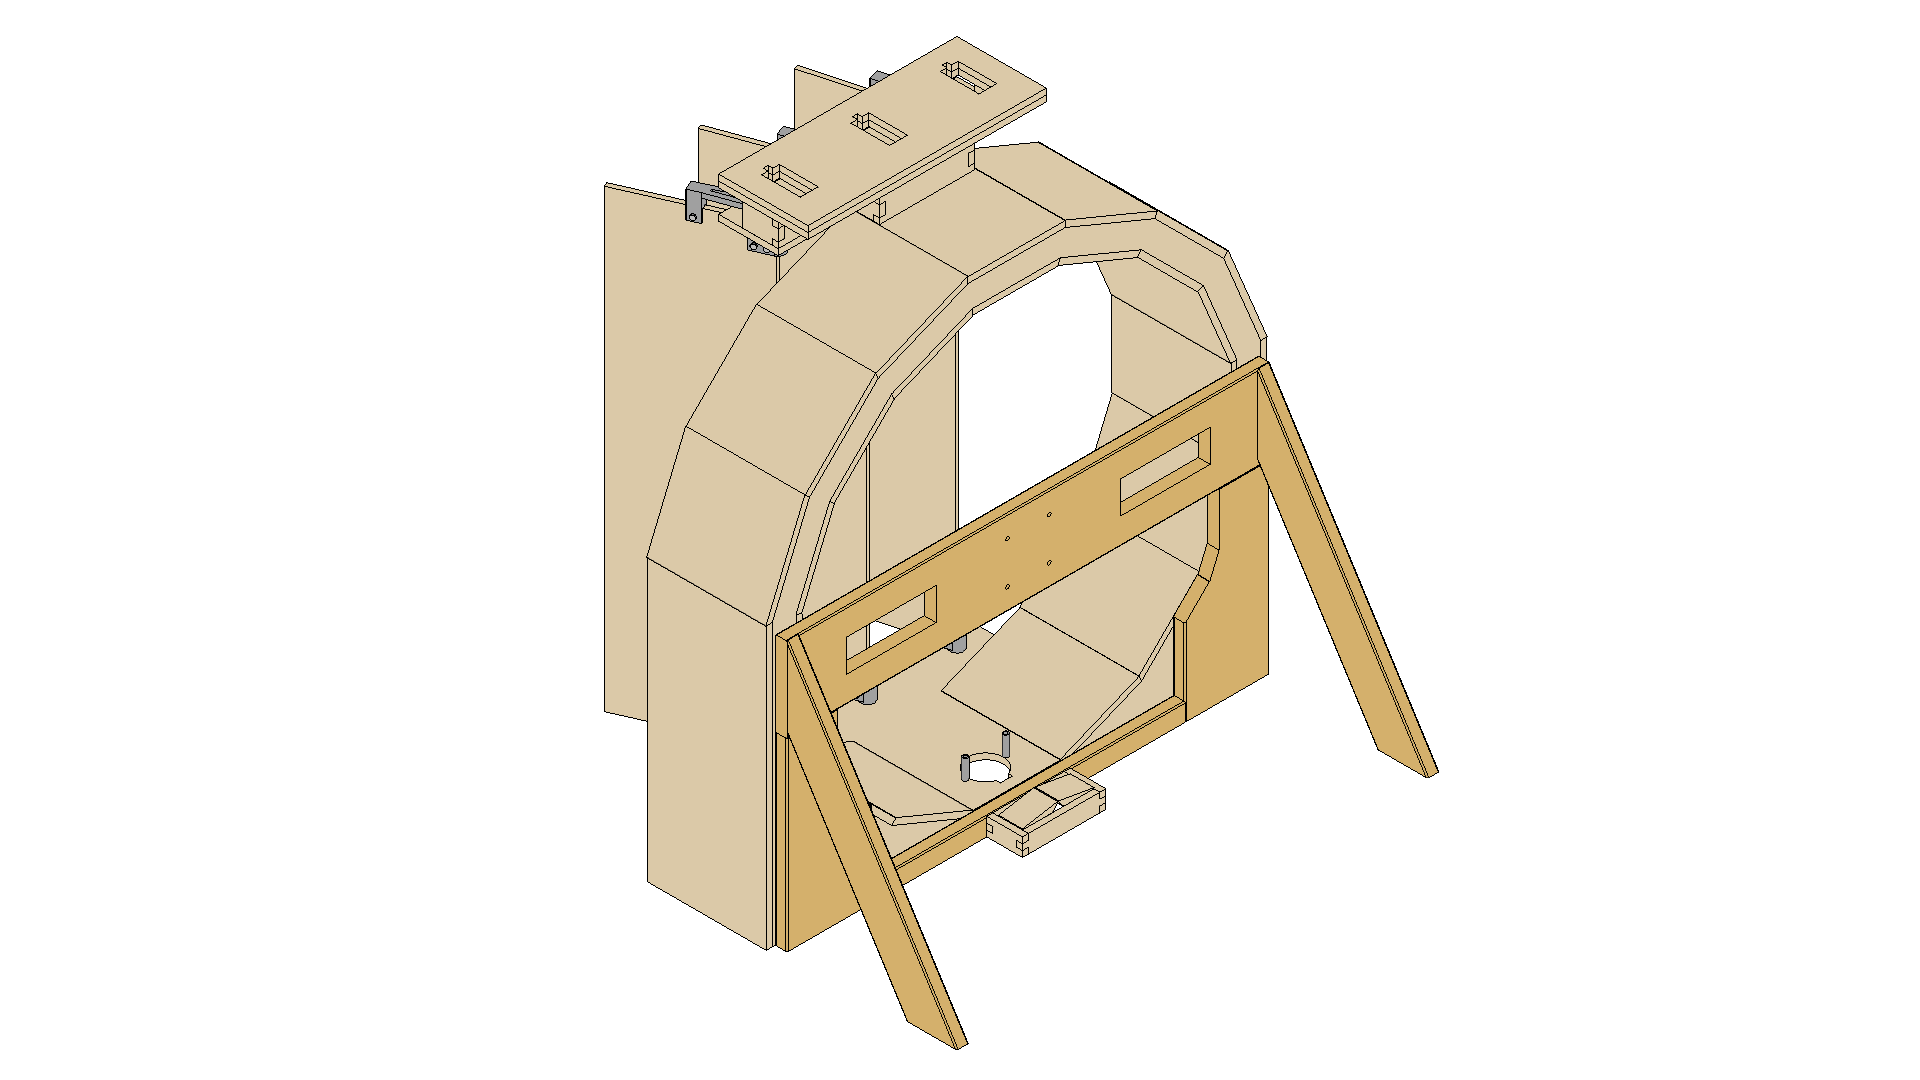
\includegraphics[width=.92\textwidth]{../Inventor/hintererAufbau/png/hintererAufbau_hinten.png}
    \caption{hinterer Aufbau Ansicht schräg hinten}
\end{figure}
\begin{figure}[H]
    \centering
    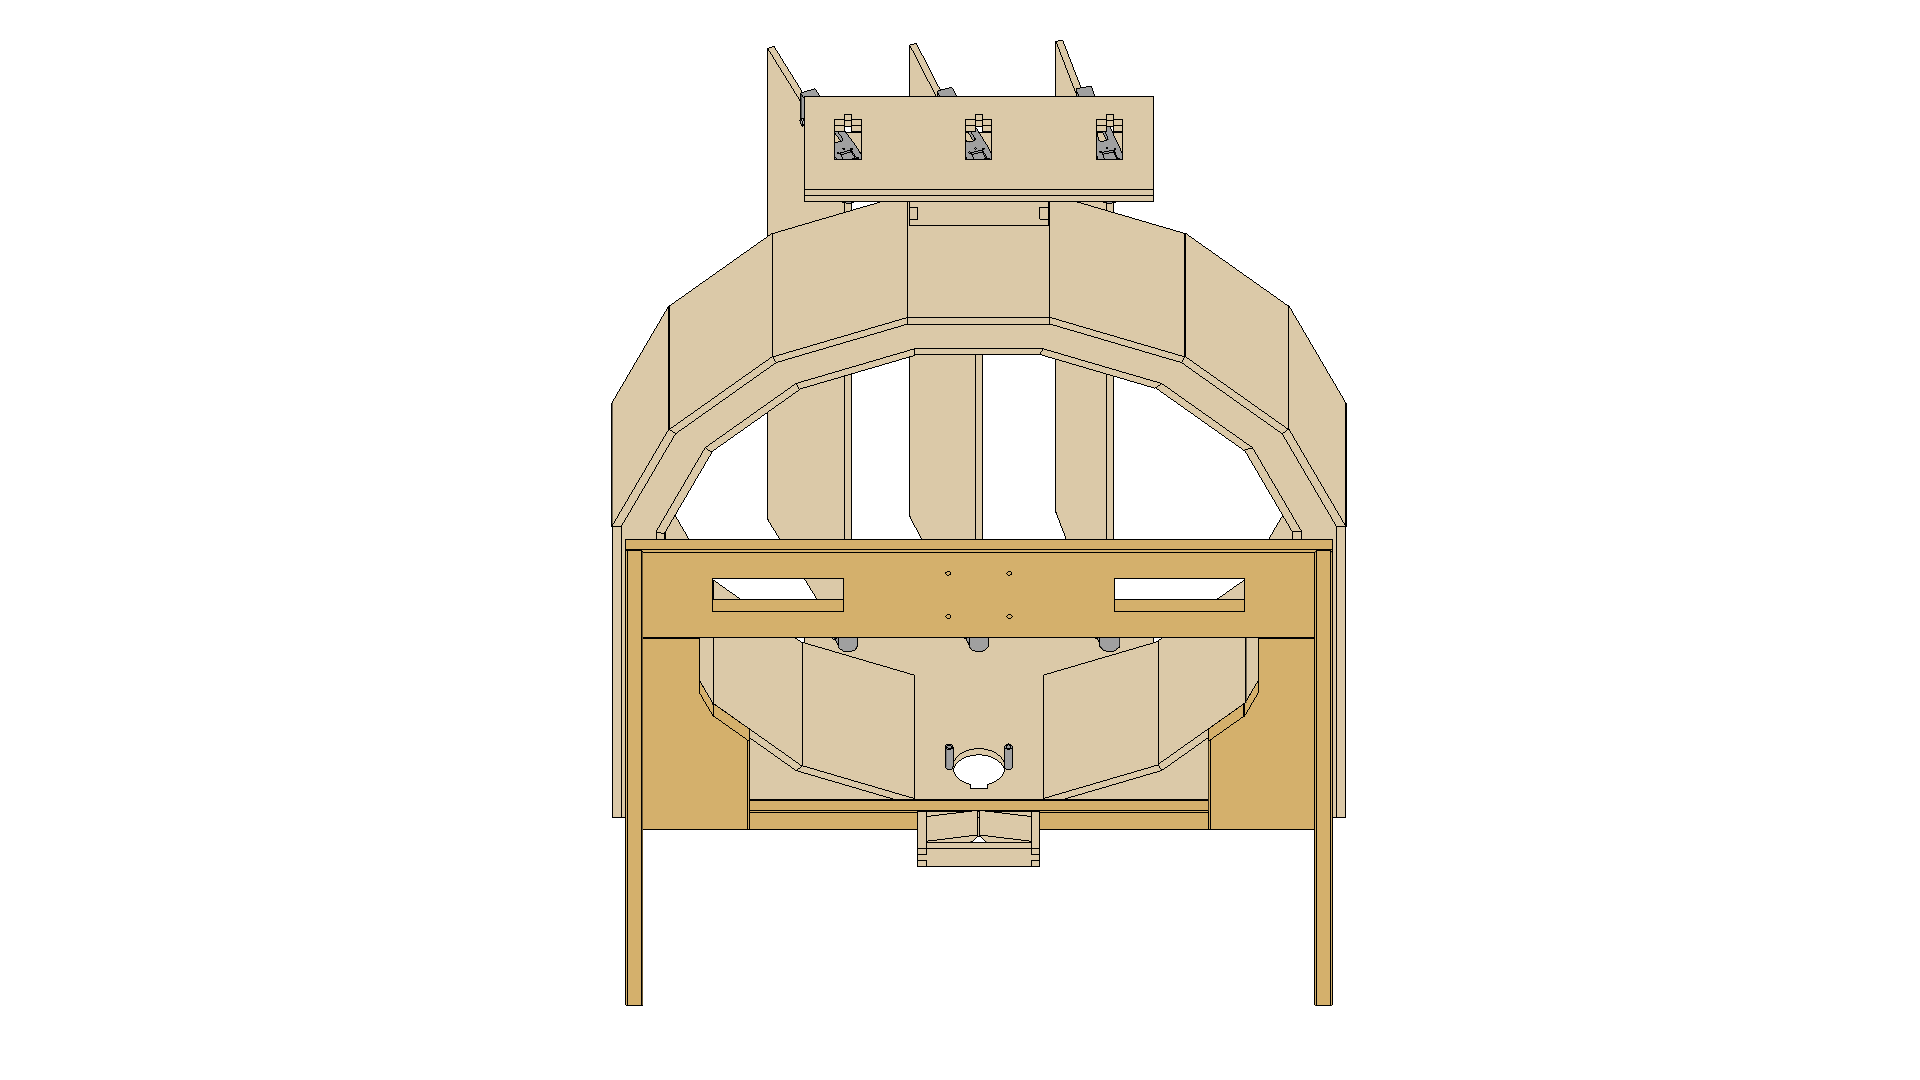
\includegraphics[width=.92\textwidth]{../Inventor/hintererAufbau/png/hintererAufbau_hintenOben.png}
    \caption{hinterer Aufbau Ansicht hinten oben}
\end{figure}

\begin{landscape}
    \includeSkizze{../Inventor/hintererAufbau/Zeichnungen/Hauptplatte.pdf}{Hauptplatte}{fig:Aufbau:skizze:hauptplatte}{1}
    \clearpage
    \includeSkizze{../Inventor/hintererAufbau/Zeichnungen/InnenUnten.pdf}{Platte innnen unten}{fig:Aufbau:skizze:innenUnten}{1}
    \clearpage
    \includeSkizze{../Inventor/hintererAufbau/Zeichnungen/PlatteInnenEineSeite.pdf}{Platte innen 1 schräge Kante}{fig:Aufbau:skizze:innen1seite}{1}
    \clearpage
    \includeSkizze{../Inventor/hintererAufbau/Zeichnungen/PlatteInnenzweiSeiten.pdf}{Platte innen 2 schräge Kanten}{fig:Aufbau:skizze:innen2seite}{1}
    \clearpage
    \includeSkizze{../Inventor/hintererAufbau/Zeichnungen/aussenOben.pdf}{Platte außen oben}{fig:Aufbau:skizze:assenOebn}{1}
    \clearpage
    \includeSkizze{../Inventor/hintererAufbau/Zeichnungen/PlatteAussenEineSeite.pdf}{Platte außen 1 schräge Kante}{fig:Aufbau:skizze:aussen1seite}{1}
    \clearpage
    \includeSkizze{../Inventor/hintererAufbau/Zeichnungen/PlatteAussenZweiSeiten.pdf}{Platte außen 2 schräge Kanten}{fig:Aufbau:skizze:assen2seite}{1}
    \clearpage
    \includeSkizze{../Inventor/hintererAufbau/Zeichnungen/PlatteAussenGross.pdf}{Platte außen Seite}{fig:Aufbau:skizze:aussengross}{1}
    \clearpage
    \includeSkizze{../Inventor/hintererAufbau/Zeichnungen/VerstaerkungHintenMitte.pdf}{Verstärkung hinten mitte}{fig:Aufbau:skizze:vhintenmitte}{1}
    \clearpage
    \includeSkizze{../Inventor/hintererAufbau/Zeichnungen/VerstaerkungHintenUnten.pdf}{Verstärkung hinten unten}{fig:Aufbau:skizze:vhintenunten}{1}
    \clearpage
    \includeSkizze{../Inventor/hintererAufbau/Zeichnungen/VerstaerkungHintenSchraeg.pdf}{Verstärkung hinten schräg}{fig:Aufbau:skizze:vhintenschraeg}{1}
    \clearpage
    \includeSkizze{../Inventor/hintererAufbau/Zeichnungen/VerstaerkungUnten.pdf}{Verstärkung unten}{fig:Aufbau:skizze:vunten}{1}
    \clearpage
    \includeSkizze{../Inventor/hintererAufbau/Zeichnungen/HalterungServosHochSeitlich.pdf}{Servo Halter seitlich}{fig:Aufbau:skizze:shs}{1}
    \clearpage
    \includeSkizze{../Inventor/hintererAufbau/Zeichnungen/HalterungServoHochSeitlich2.pdf}{Servo Halter seitlich 2}{fig:Aufbau:skizze:shs2}{1}
    \clearpage
    \includeSkizze{../Inventor/hintererAufbau/Zeichnungen/HolzServoHalterHinten.pdf}{Servo Halter hinten}{fig:Aufbau:skizze:shh}{1}
    \clearpage
    \includeSkizze{../Inventor/hintererAufbau/Zeichnungen/HolzServoHalterHochLang.pdf}{Servo Halter lang}{fig:Aufbau:skizze:shl}{1}
    \clearpage
    \includeSkizze{../Inventor/hintererAufbau/Zeichnungen/HolzServoHalterMainPlatte1.pdf}{Servo Halter Hauptplatte}{fig:Aufbau:skizze:shhp}{1}
    \clearpage
    \includeSkizze{../Inventor/hintererAufbau/Zeichnungen/KabelBoxPlatteKurz.pdf}{Kabelbox Platte kurz}{fig:Aufbau:skizze:kbk}{1}
    \clearpage
    \includeSkizze{../Inventor/hintererAufbau/Zeichnungen/KabelBoxPlatteLang.pdf}{Kabelbox Platte lang}{fig:Aufbau:skizze:kbl}{1}
    \clearpage
    \includeSkizze{../Inventor/hintererAufbau/Zeichnungen/KabelBoxDeckel.pdf}{Kabelbox Deckel}{fig:Aufbau:skizze:kbd}{1}
    \clearpage

    \includeSkizze{../Inventor/hintererAufbau/Zeichnungen/Fahnen_Halter_hauptteil.pdf}{Fahnenhalter Hauptteil}{fig:Aufbau:skizze:fhh}{1}
    \clearpage
    \includeSkizze{../Inventor/hintererAufbau/Zeichnungen/Fahnen_Halter_obenTeileServo.pdf}{Fahnenhalter Servo}{fig:Aufbau:skizze:fhs}{1}
    \clearpage
    \includeSkizze{../Inventor/hintererAufbau/Zeichnungen/Fahnen_Halter_rechteck.pdf}{Fahnenhalter Rechteck}{fig:Aufbau:skizze:fhr}{1}
    \clearpage
    
\end{landscape}

\subsection{Zusammenbau}
Der hintere Aufbau wurde, wie in Inventor geplant, aufgebaut und mit 16 Stück 70x70x55mm Winkelverbinder mit der Bodenplatte verbunden. Zusätzlich sind die schrägen Verstärkungen (\autoref{fig:Aufbau:skizze:vhintenschraeg}) mit je 2 Stück 50x50x35mm Winkelverbinder befestigt.\\
Die Winkelverbinder sind mit Holzschrauben an der Bodenplatte fix befestigt. Der hintere Aufbau wird mit 10 Stück M8 Schrauben an den Winkelverbindern festgeschraubt und ist somit relativ leicht abnehmbar.\\
Die Löcher für die M8 Schrauben sind in den Zeichnungen nicht ersichtlich, da diese erst beim Zusammenbauen gebohrt wurden, um eine gute Passgenauigkeit zu garantieren.\\
\begin{figure}[H]
    \centering
    \missingfigure{Zusammenbau hinterer Aufbau Foto machen (ev. von 2 Perspektiven oder mehr)}
    \caption{Zusammenbau hinterer Aufbau}
\end{figure}

\clearpage
\section{Lenkung}
Die Lenkung beinhaltet die komplette Steuerung des Hovercrafts.\\
Der Lenker selbst ist ein Fahrrad-Lenker, welcher auf einer Metallstange befestigt wird. Diese Metallstange muss so stabil sein, damit sich der Fahrer an der Lenkung festhalten kann. Die Lenkerstellung wird mit einem Potenziometer, welches ebenfalls in der Box verbaut ist, ausgelesen.\\
An dem Fahrradlenker ist zusätzlich zu den beiden Daumengashebeln noch ein Display montiert, um alle für den Fahrer wichtigen Informationen anzuzeigen.\\
Um den Lenker automatisch zu zentrieren und der Lenkung ein Gegenmoment zu geben, wurden Federn verwendet.
\begin{figure}[H]
    \centering
    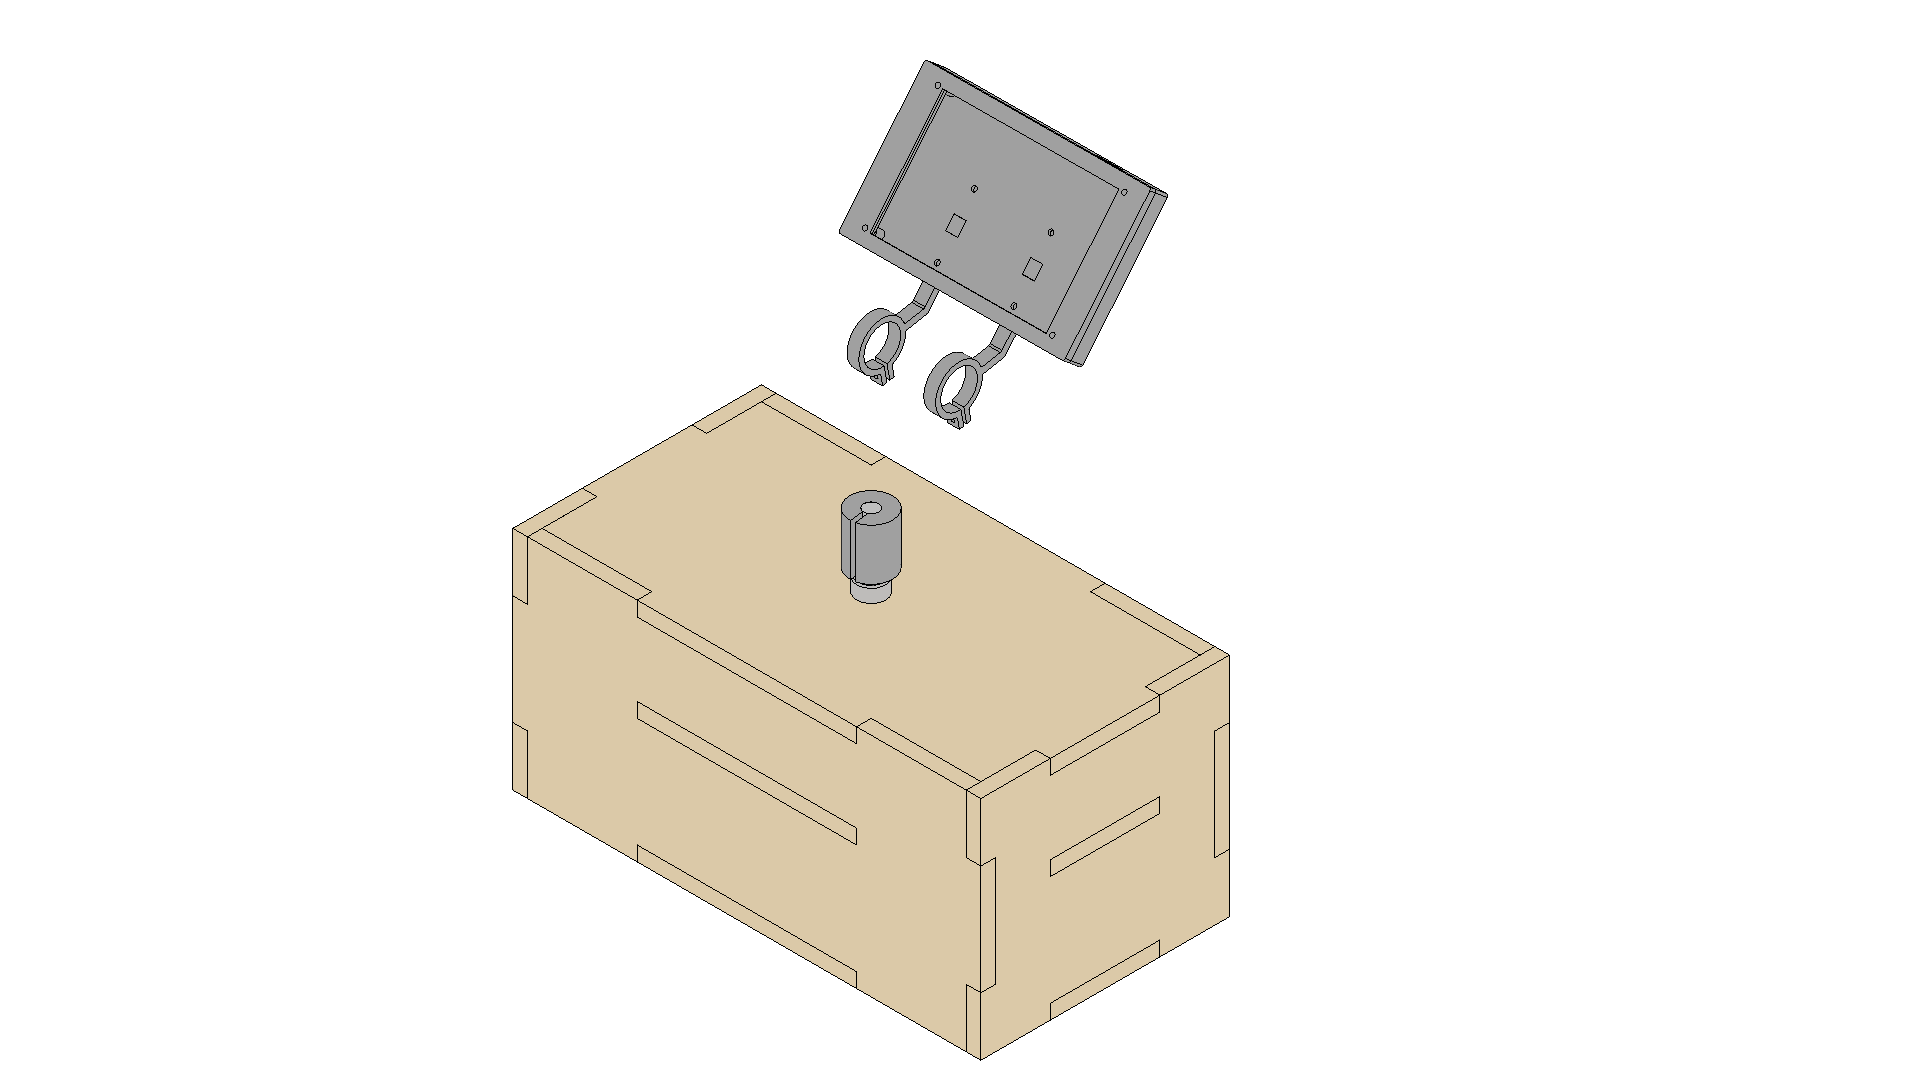
\includegraphics[width=1.25\textwidth]{../Inventor/Lenker/png/Lenkung_Hauptansicht.png}
    \caption{Lenkung 3D-Modell}
\end{figure}

\clearpage
\subsection{Stückliste}
\todo{Lenker - Amazon}
\begin{table}[H]
    \centering
    \begin{tabular}{|c|M{4.5cm}|M{3.5cm}|c|c|}
        \hline
        \textbf{Stk} & \textbf{Name} & \textbf{Material} & \textbf{Herstellung} & \textbf{Abbildung}\\\hline
        1 & Bodenplatte & 10mm Pappel & LaserCutter & \ref{fig:Lenkung:skizze:bodenplatte}\\\hline
        2 & Platte Groß mit Loch & 10mm Pappel & LaserCutter & \ref{fig:Lenkung:skizze:pgl}\\\hline
        2 & Platte Seite Lang & 10mm Pappel & LaserCutter & \ref{fig:Lenkung:skizze:psl}\\\hline
        2 & Platte Seite Kurz & 10mm Pappel & LaserCutter & \ref{fig:Lenkung:skizze:psk}\\\hline
        1 & Halterung Poti unten & PETG & 3D-Drucker & \ref{fig:Lenkung:skizze:psk}\\\hline
        1 & Adapter Poti Teil 1 & PETG & 3D-Drucker & \ref{fig:Lenkung:skizze:apt1}\\\hline
        1 & Adapter Poti Teil 2 & PETG & 3D-Drucker & \ref{fig:Lenkung:skizze:apt2}\\\hline
        1 & Adapter Lenker & PETG & 3D-Drucker & \ref{fig:Lenkung:skizze:al}\\\hline
        1 & Stange Mitte & \diameter 10mm Alu-Stange & Gekauft & \ref{fig:Lenkung:skizze:sm}\\\hline
        1 & Gewindestange & M4 Gewindestange & Gekauft & \ref{fig:Lenkung:skizze:gs}\\\hline
        2 & Displayhalterung Halterung & PETG & 3D-Drucker & \ref{fig:Lenkung:skizze:nhh}\\\hline
        1 & Displayhalterung Hauptteil & PETG & 3D-Drucker & \ref{fig:Lenkung:skizze:nhm}\\\hline
        1 & Displayhalterung Deckel & PETG & 3D-Drucker & \ref{fig:Lenkung:skizze:nhd}\\\hline
    \end{tabular}
    \caption{Stückliste Aufbau hinten}
    \label{tab:konst:lenkung:stueckliste}
\end{table}

\clearpage
\subsection{Inventor}
\begin{figure}[H]
    \centering
    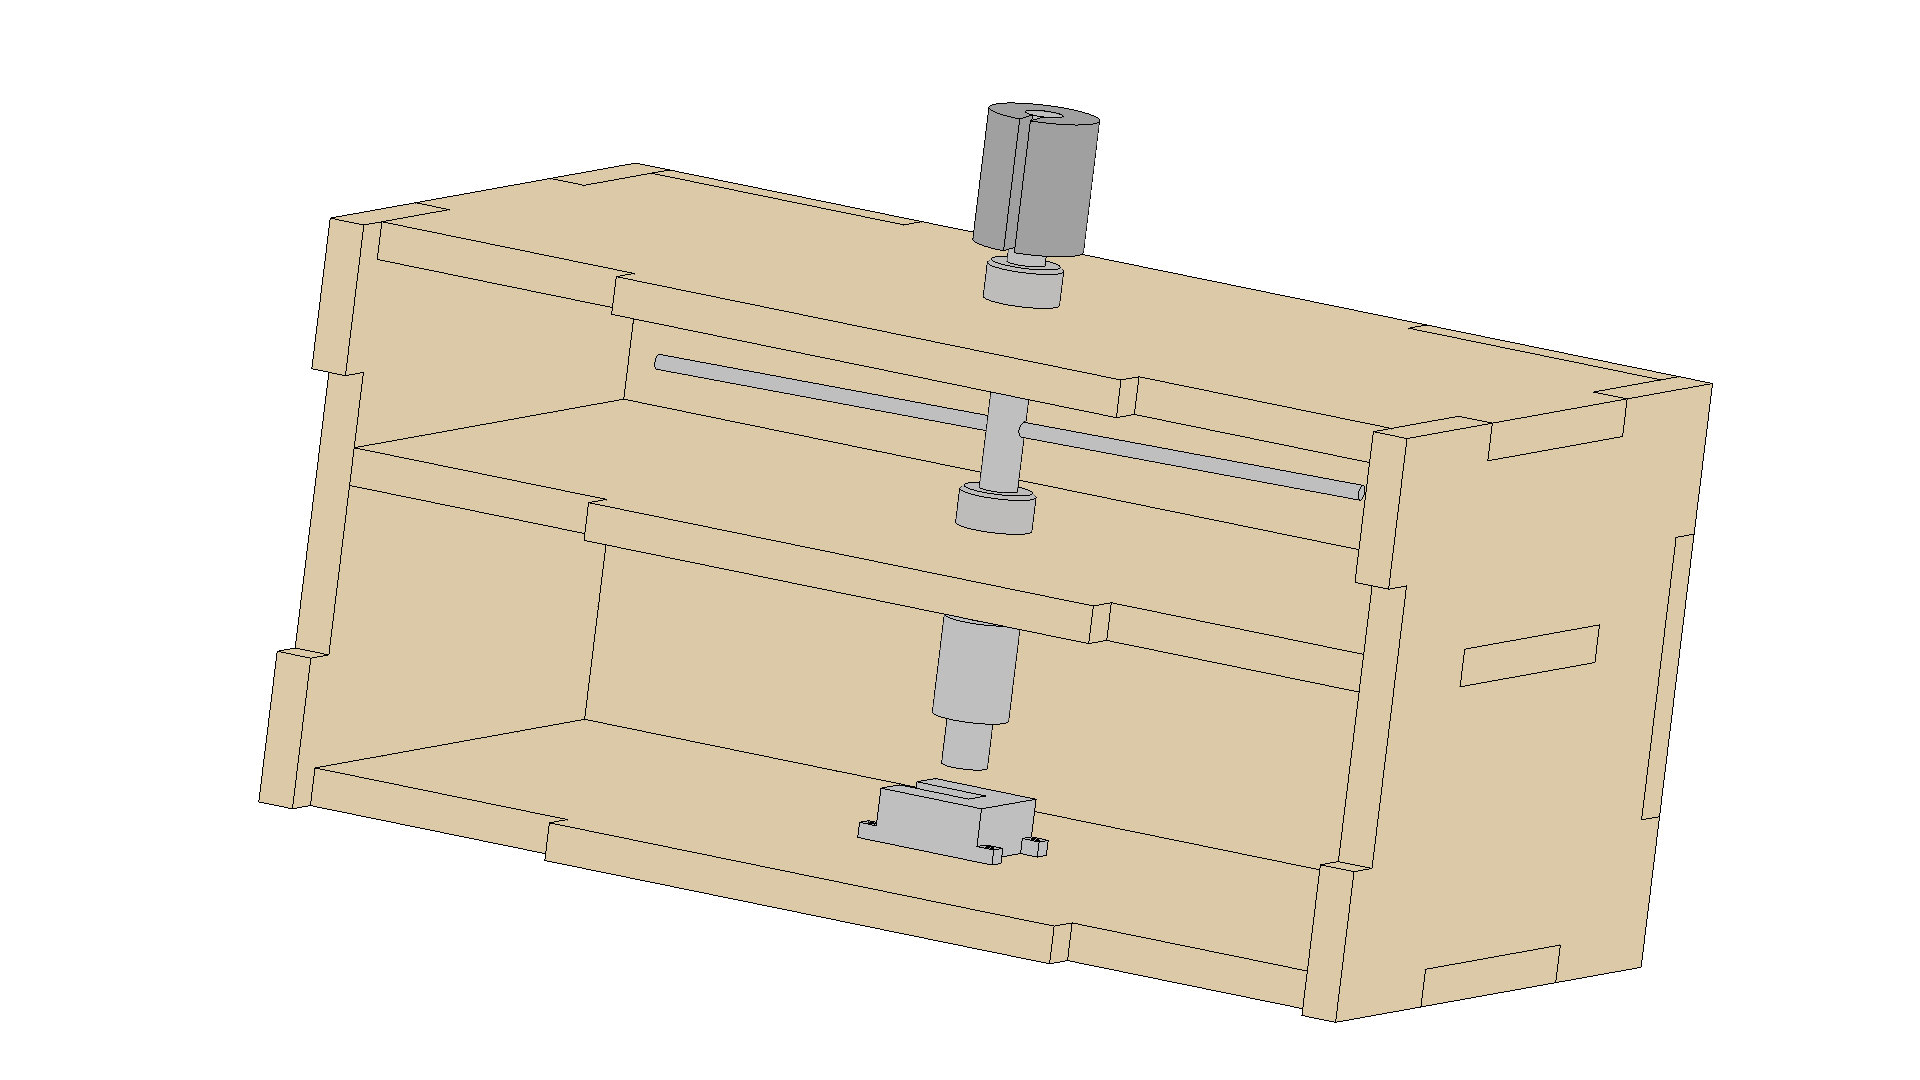
\includegraphics[width=.99\textwidth]{../Inventor/Lenker/png/Lenkung_offen.png}
    \caption{Lenkung Ansicht vorne, offen}
\end{figure}
\begin{figure}[H]
    \centering
    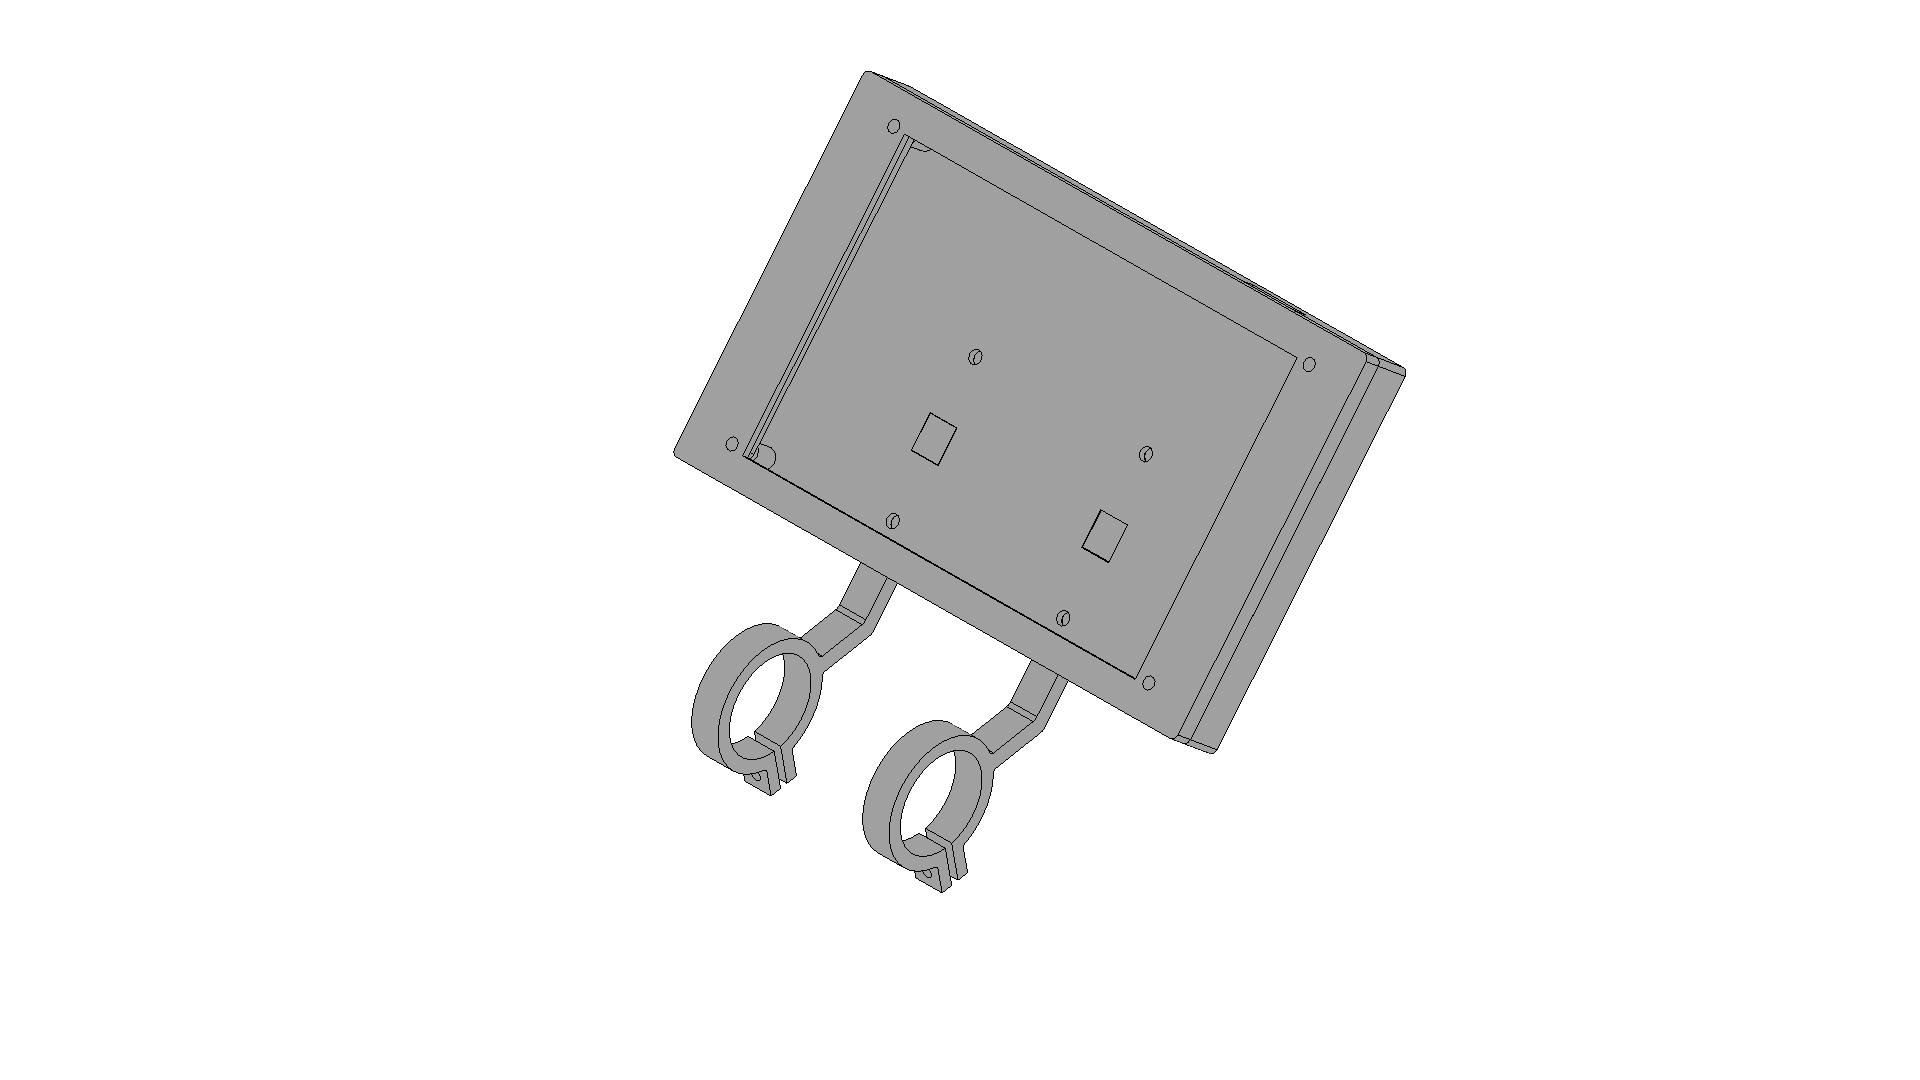
\includegraphics[width=.99\textwidth]{../Inventor/Lenker/png/Lenkung_Display.png}
    \caption{Lenkung Ansicht Display-Halterung}
\end{figure}

\begin{landscape}
    \includeSkizze{../Inventor/Lenker/Zeichnungen/Bodenplatte.pdf}{Bodenplatte}{fig:Lenkung:skizze:bodenplatte}{1}
    \clearpage
    \includeSkizze{../Inventor/Lenker/Zeichnungen/PlatteGrossLoch.pdf}{Platte Groß mit Loch}{fig:Lenkung:skizze:pgl}{1}
    \clearpage
    \includeSkizze{../Inventor/Lenker/Zeichnungen/PlatteSeiteLang.pdf}{Platte Seite Lang}{fig:Lenkung:skizze:psl}{1}
    \clearpage
    \includeSkizze{../Inventor/Lenker/Zeichnungen/PlatteSeiteKurz.pdf}{Platte Seite Kurz}{fig:Lenkung:skizze:psk}{1}
    \clearpage

    \includeSkizze{../Inventor/Lenker/Zeichnungen/PotiHalterungUnten.pdf}{Poti Halterung}{fig:Lenkung:skizze:poth}{1}
    \clearpage

    \includeSkizze{../Inventor/Lenker/Zeichnungen/AdapterPoti1.pdf}{Adapter Poti Teil 1}{fig:Lenkung:skizze:apt1}{1}
    \clearpage
    \includeSkizze{../Inventor/Lenker/Zeichnungen/AdapterPoti2.pdf}{Adapter Poti Teil 2}{fig:Lenkung:skizze:apt2}{1}
    \clearpage

    \includeSkizze{../Inventor/Lenker/Zeichnungen/AdapterLenker.pdf}{Adapter Lenker}{fig:Lenkung:skizze:al}{1}
    \clearpage

    \includeSkizze{../Inventor/Lenker/Zeichnungen/StangeMitte.pdf}{Stange Mitte}{fig:Lenkung:skizze:sm}{1}
    \clearpage

    \includeSkizze{../Inventor/Lenker/Zeichnungen/M4Gewindestange.pdf}{Gewindestange}{fig:Lenkung:skizze:gs}{1}
    \clearpage

    \includeSkizze{../Inventor/Lenker/Zeichnungen/Mount_Nextion_Display_Halter.pdf}{Displayhalterung Halterung}{fig:Lenkung:skizze:nhh}{1}
    \clearpage
    \includeSkizze{../Inventor/Lenker/Zeichnungen/Mount_Nextion_Display_Main.pdf}{Displayhalterung Hauptteil}{fig:Lenkung:skizze:nhm}{1}
    \clearpage
    \includeSkizze{../Inventor/Lenker/Zeichnungen/Mount_Nextion_Display_Deckel.pdf}{Displayhalterung Deckel}{fig:Lenkung:skizze:nhd}{1}
    \clearpage
\end{landscape}



\cleardoublepage
\subsection{Zusammenbau}
Die Lenkung wurde, wie in Inventor geplant, zusammengebaut. Die Löcher für den Not-Aus, den Precharge-Taster und die Kabel des Displays und der Daumengashebel wurden gebohrt.\\
Um die 4 Federn, welchen den Lenker zentrieren, befestigen und spannen zu können, wurden M6 Schrauben verwendet -- siehe \autoref{fig:lenkung:federsys}.\\
Die Lenkung ist wie der hintere Aufbau ebenfalls mit 4 Stück 50x50x35mm Winkelverbinder an der Bodenplatte befestigt.
\begin{figure}[H]
    \centering
    \missingfigure{Foto Federung Lenkung machen}
    \caption{Foto Federsystem Lenkung \label{fig:lenkung:federsys}}
\end{figure}
\begin{figure}[H]
    \centering
    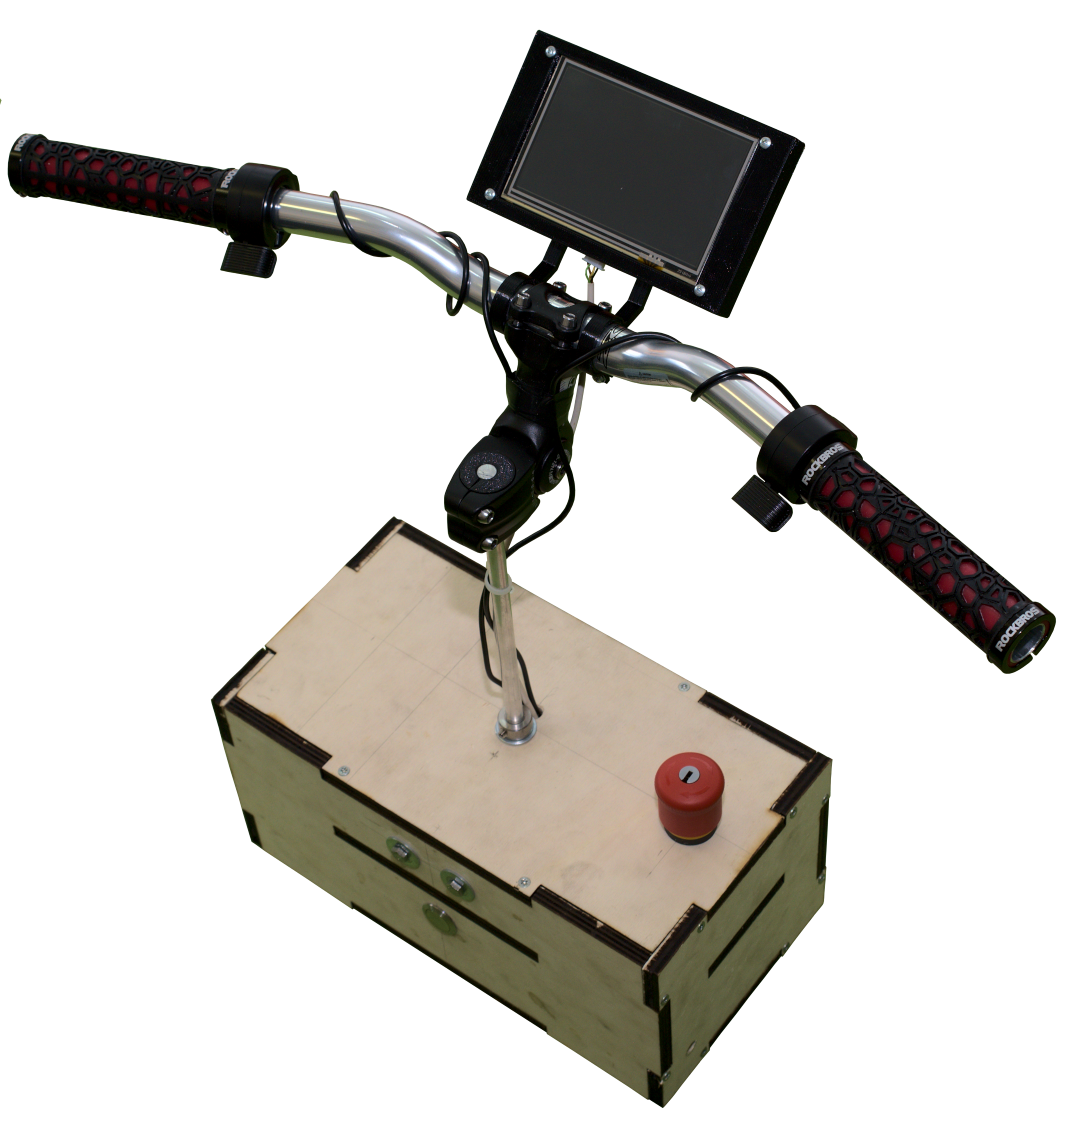
\includegraphics[width=.99\textwidth]{Fotos/Konstruktion/DSC_8590.png}
    \caption{Zusammenbau Lenkung}
\end{figure}

\clearpage
\section{Zusammenbau}
Die Konstruktion wurde wie in den Unterkapiteln bereits beschrieben zusammengebaut.\\
Zusätzlich wurden Sticker mit den Logos der Sponsoren angebracht.
\begin{figure}[H]
    \centering
    \missingfigure{Fotos (2) gesamter Zusammenbau machen (ev. draussen mit schönem Hintergrund)}
    \caption{gesamter Zusammenbau}
\end{figure}

